\documentclass[manuscript,screen,nonacm]{acmart}
\usepackage{amsmath}
\usepackage{color,soul}
\usepackage{tikz}
\usetikzlibrary{positioning}
\usepackage{pgfplots}
\pgfplotsset{width=7cm, compat=1.9}
\usepackage{pgf-pie}
\usetikzlibrary{trees}
\usepackage{xcolor}
\usepackage[utf8]{inputenc}
\usepackage[T1]{fontenc}

\begin{document}

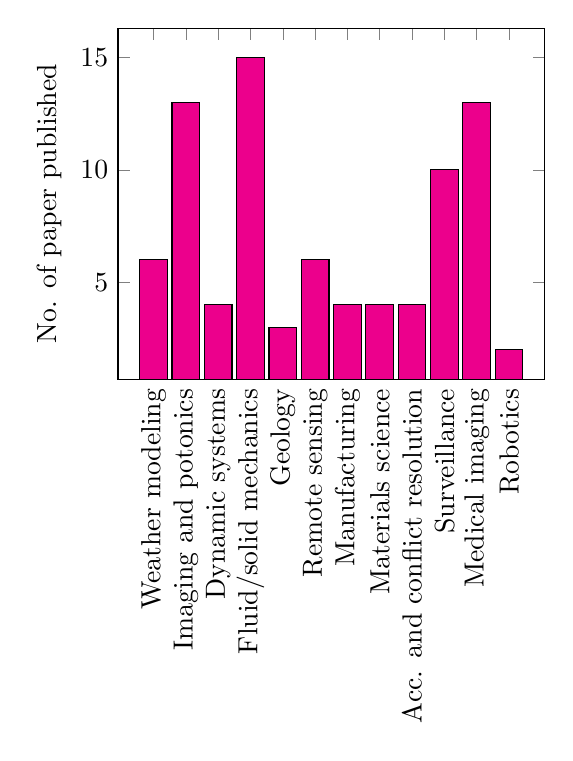
\begin{tikzpicture}[scale=1]
    \begin{axis}[
        symbolic x coords={Weather modeling, Imaging and potonics, Dynamic systems, Fluid/solid mechanics, Geology, Remote sensing, Manufacturing, Materials science, Acc. and conflict resolution, Surveillance, Medical imaging, Robotics}, 
        xtick={Weather modeling, Imaging and potonics, Dynamic systems, Fluid/solid mechanics, Geology, Remote sensing, Manufacturing, Materials science, Acc. and conflict resolution, Surveillance, Medical imaging, Robotics}, 
        x tick label style={rotate=90,anchor=east}, 
        ylabel= No. of paper published]

        \addplot[ybar,fill=magenta] coordinates {
            (Weather modeling,6)
            (Imaging and potonics,13)
            (Dynamic systems,4)
            (Fluid/solid mechanics,15)
            (Geology,3)
            (Remote sensing,6)
            (Manufacturing,4)
            (Materials science,4)
            (Acc. and conflict resolution,4)
            (Surveillance,10)
            (Medical imaging,13)
            (Robotics,2)

        };

    \end{axis}
    \end{tikzpicture}

\end{document}